%% This file was auto-generated by IPython.
%% Conversion from the original notebook file:
%% logreg.ipynb
%%
\documentclass[11pt,english,fleqn]{article}

%% This is the automatic preamble used by IPython.  Note that it does *not*
%% include a documentclass declaration, that is added at runtime to the overall
%% document.

\usepackage{amsmath}
\usepackage{amssymb}
\usepackage{graphicx}
\usepackage{ucs}
\usepackage[utf8x]{inputenc}

% needed for markdown enumerations to work
\usepackage{enumerate}

% Slightly bigger margins than the latex defaults
\usepackage{geometry}
\geometry{verbose,tmargin=3cm,bmargin=3cm,lmargin=2.5cm,rmargin=2.5cm}

% Define a few colors for use in code, links and cell shading
\usepackage{color}
\definecolor{orange}{cmyk}{0,0.4,0.8,0.2}
\definecolor{darkorange}{rgb}{.71,0.21,0.01}
\definecolor{darkgreen}{rgb}{.12,.54,.11}
\definecolor{myteal}{rgb}{.26, .44, .56}
\definecolor{gray}{gray}{0.45}
\definecolor{lightgray}{gray}{.95}
\definecolor{mediumgray}{gray}{.8}
\definecolor{inputbackground}{rgb}{.95, .95, .85}
\definecolor{outputbackground}{rgb}{.95, .95, .95}
\definecolor{traceback}{rgb}{1, .95, .95}

% Framed environments for code cells (inputs, outputs, errors, ...).  The
% various uses of \unskip (or not) at the end were fine-tuned by hand, so don't
% randomly change them unless you're sure of the effect it will have.
\usepackage{framed}

% remove extraneous vertical space in boxes
\setlength\fboxsep{0pt}

% codecell is the whole input+output set of blocks that a Code cell can
% generate.

% TODO: unfortunately, it seems that using a framed codecell environment breaks
% the ability of the frames inside of it to be broken across pages.  This
% causes at least the problem of having lots of empty space at the bottom of
% pages as new frames are moved to the next page, and if a single frame is too
% long to fit on a page, will completely stop latex from compiling the
% document.  So unless we figure out a solution to this, we'll have to instead
% leave the codecell env. as empty.  I'm keeping the original codecell
% definition here (a thin vertical bar) for reference, in case we find a
% solution to the page break issue.

%% \newenvironment{codecell}{%
%%     \def\FrameCommand{\color{mediumgray} \vrule width 1pt \hspace{5pt}}%
%%    \MakeFramed{\vspace{-0.5em}}}
%%  {\unskip\endMakeFramed}

% For now, make this a no-op...
\newenvironment{codecell}{}

 \newenvironment{codeinput}{%
   \def\FrameCommand{\colorbox{inputbackground}}%
   \MakeFramed{\advance\hsize-\width \FrameRestore}}
 {\unskip\endMakeFramed}

\newenvironment{codeoutput}{%
   \def\FrameCommand{\colorbox{outputbackground}}%
   \vspace{-1.4em}
   \MakeFramed{\advance\hsize-\width \FrameRestore}}
 {\unskip\medskip\endMakeFramed}

\newenvironment{traceback}{%
   \def\FrameCommand{\colorbox{traceback}}%
   \MakeFramed{\advance\hsize-\width \FrameRestore}}
 {\endMakeFramed}

% Use and configure listings package for nicely formatted code
\usepackage{listingsutf8}
\lstset{
  language=python,
  inputencoding=utf8x,
  extendedchars=\true,
  aboveskip=\smallskipamount,
  belowskip=\smallskipamount,
  xleftmargin=2mm,
  breaklines=true,
  basicstyle=\small \ttfamily,
  showstringspaces=false,
  keywordstyle=\color{blue}\bfseries,
  commentstyle=\color{myteal},
  stringstyle=\color{darkgreen},
  identifierstyle=\color{darkorange},
  columns=fullflexible,  % tighter character kerning, like verb
}

% The hyperref package gives us a pdf with properly built
% internal navigation ('pdf bookmarks' for the table of contents,
% internal cross-reference links, web links for URLs, etc.)
\usepackage{hyperref}
\hypersetup{
  breaklinks=true,  % so long urls are correctly broken across lines
  colorlinks=true,
  urlcolor=blue,
  linkcolor=darkorange,
  citecolor=darkgreen,
  }

% hardcode size of all verbatim environments to be a bit smaller
\makeatletter 
\g@addto@macro\@verbatim\small\topsep=0.5em\partopsep=0pt
\makeatother 

% Prevent overflowing lines due to urls and other hard-to-break entities.
\sloppy

\setlength{\mathindent}{0pt}
\setlength{\parindent}{0pt}
\setlength{\parskip}{8pt}
\begin{document}

Lojistik Regresyon (Logistic Regression)

Lojistik regresyon normal regresyonun $\theta^T x$ olarak kullandigi
agirliklar (katsayilar) ile verinin carpimini alir ve ek bir filtre
fonksiyonundan gecirerek onlari 0/1 degerleri baglaminda bir olasiliga
esler. Yani elimizdeki veri pek cok boyutta veri noktalari ve o
noktalarin 0 ya da 1 olarak bir ``etiketi'' olacaktir. Mesela

\begin{codecell}
\begin{codeinput}
\begin{lstlisting}
from pandas import *
df = read_csv("testSet.txt",sep='\t',names=['x','y','labels'],header=None)
df['intercept']=1.0
data = df[['intercept','x','y']]
labels = df['labels']
df[['x','y','labels']][:10]

\end{lstlisting}
\end{codeinput}
\begin{codeoutput}
\begin{verbatim}
          x          y  labels
0 -0.017612  14.053064       0
1 -1.395634   4.662541       1
2 -0.752157   6.538620       0
3 -1.322371   7.152853       0
4  0.423363  11.054677       0
5  0.406704   7.067335       1
6  0.667394  12.741452       0
7 -2.460150   6.866805       1
8  0.569411   9.548755       0
9 -0.026632  10.427743       0
\end{verbatim}
\end{codeoutput}
\end{codecell}
Goruldugu gibi veride $x,y$ boyutlari icin etiketler (labels) verilmis.
Lojistik regresyon bu veriyi kullanarak egitim sonrasi $\theta$'lari
elde eder, bunlar katsayilarimizdir, artik bu katsayilari hic
gormedigimiz yeni bir veri uzerinde 0/1 etiketlerinin tahminini yapmak
icin kullanabiliriz.

Filtre fonksiyonu icin kullanilan bir fonksiyon sigmoid fonksiyonudur,
$g(x)$ ismini verelim,
\[ g(x) = \frac{e^{x}}{1+e^{x}} \]
Bu nasil bir fonksiyondur, kabaca davranisini nasil tarif ederiz?
Cebirsel olarak bakarsak, fonksiyon oyle bir durumda ki ne zaman bir $x$
degeri gecersek, bu deger ne kadar buyuk olursa olsun, bolendeki deger
her zaman bolunenden 1 daha fazla olacaktir bu da fonksiyonun sonucunun
1'den her zaman kucuk olmasini garantiler. Cok kucuk $x$ degerleri icin
bolum sonucu biraz daha buyuk olacaktir tabii, vs.

Daha temiz bir ifade icin bolen ve boluneni $e^{-x}$ ile carpalim,
\[ g(x) = \frac{e^{x}e^{-x}}{e^{-x}+e^{x}e^{-x}} \]\[ g(x) = \frac{1}{1+e^{-x}} \]
Sigmoid fonksiyonun ``-sonsuzluk ile +sonsuzluk arasindaki degerleri 0
ve 1 arasina esledigi / indirgedigi (map)'' ifadesi de litaraturde
mevcuttur.

\begin{codecell}
\begin{codeinput}
\begin{lstlisting}
def sigmoid(arr):
    return 1.0/(1+exp(-arr))

x = np.array(arange(-10.0, 10.0, 0.1))
plot(x,sigmoid(x))
    
\end{lstlisting}
\end{codeinput}
\begin{codeoutput}
\begin{verbatim}
[<matplotlib.lines.Line2D at 0x9cfcd2c>]
\end{verbatim}
\begin{center}
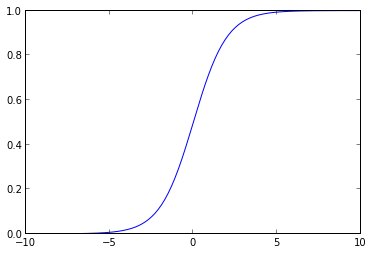
\includegraphics[width=0.7\textwidth]{logreg_files/logreg_fig_00.png}
\par
\end{center}
\end{codeoutput}
\end{codecell}
Ustteki grafige bakinca katsayilarla carpim, toplam ardindan sonucun
niye bu fonksiyona verildigini anlamak mumkun. Sigmoid'in 0 seviyesinden
1 seviyesine ziplayisi oldukca hizli ve $x$ kordinati baglaminda (ve
0.5'ten kucuk $y$'ye eslenen) sifir oncesi bolgesi, ayni sekilde sifir
sonrasi (ve 0.5'ten buyuk $y$'ye eslenen) bolgesi oldukca buyuk. Yani bu
fonksiyonu secmekle veriye katsayilarla carpilip 0 ya da 1 bolgesi
altina dusmesi icin oldukca genis bir sans veriyoruz. Boylece veriyi iki
parcaya ayirmak icin sansimizi arttirmis oluyoruz.

Peki sigmoid fonksiyonu bir olasilik fonksiyonu (dagilimi) olarak
kullanilabilir mi? Entegralini alalim, ve -/+ sonsuzluklar uzerinden
alan hesabi yapalim, sonucun 1 cikmasi gerekli,

\begin{codecell}
\begin{codeinput}
\begin{lstlisting}
import sympy
x = sympy.Symbol('x')
sympy.integrate('1/(1+exp(-x))')

\end{lstlisting}
\end{codeinput}
\begin{codeoutput}
\begin{verbatim}
x + log(1 + exp(-x))
\end{verbatim}
\end{codeoutput}
\end{codecell}
Daha temizlemek icin
\[ x + \ln(1 + e^{-x}) \]
$x$ ifadesi ayni zamanda suna esittir $x=ln( e^{x} )$. Bu ifade bize
kolaylik saglayacak boylece,
\[ \ln e^{x} + \ln(1+e^{-x})  \]
diyebiliriz. Dogal log'un (ln) carpimlari toplamlara donusturdugunu
biliyoruz, bunu tersinden uygulayalim,
\[ \ln (e^{x}\cdot 1 + e^{x}e^{-x})  \]\[ \ln (e^{x} + 1)  = \ln (1 + e^{x} )  \]
\begin{codecell}
\begin{codeinput}
\begin{lstlisting}
print log (1+exp(-inf))
print log(1+exp(inf))
\end{lstlisting}
\end{codeinput}
\begin{codeoutput}
\begin{verbatim}
0.0
inf
\end{verbatim}
\end{codeoutput}
\end{codecell}
Demek ki fonksiyon bir olasilik dagilimi olamaz, cunku egri altindaki
alan sonsuz buyuklugunde. Aslinda bu fonksiyonun kumulatif dagilim
fonksiyonu (cumulative distribution function -CDF-) ozellikleri vardir,
yani kendisi degil ama turevi bir olasilik fonksiyonu olarak
kullanilabilir (bu konumuz disinda).

Her neyse, sigmoid'in bir CDF gibi hareket ettigini $g$'nin 0 ile 1
arasinda olmasindan da anliyoruz, sonucta CDF alan demektir (yogunlugun
entegrali) ve en ust degeri 1 demektir, ki bu CDF tanimina uygundur.

Simdi elimizde olabilecek $k$ tane degisken ve bu degiskenlerin
bilinmeyen katsayilari icin 0 ve 1'e eslenecek bir regresyon
olusturalim. Diyelim ki katsayilar $\theta_0,..,\theta_k$. Bu
katsayilari degiskenler ile carpip toplayarak $h(x)$'e verelim, (0/1)
cikip cikmayacagi katsayilara bagli olacak, verideki etiketler ile
$h(x)$ sonucu arasinda bir baglanti kurabilirsek, bu bize katsayilari
verebilir. Bu modele gore eger $\theta$'yi ne kadar iyi secersek, eldeki
veriye etiketlerine o kadar yaklasmis olacagiz. Simdi sigmoid'i
katsayilarla beraber yazalim,
\[ h_\theta(x) = g(\theta^T x) = \frac{1}{1+e^{-\theta^T x}} \]
``Veriye olabildigince yaklasmak icin en iyi $\alpha$'yi bulmak'' sozu
bize maksimum olurluk (maximum likelihood) hesabini hatirlatmali. Bu
hesaba gore icinde bilinmeyen $\alpha$'yi barindiran formulun uzerinden
tum verinin sonuclarinin teker teker birbiri ile carpimi olabildigince
buyuk olmalidir. Bu ifadeyi maksimize edecek $\alpha$ veriye en uygun
$\alpha$ olacaktir.

Simdi her iki etiket icin ve sigmoid'i kullanarak olasilik hesaplarini
yapalim,
\[ P(y=1 | x;\theta) = h_\theta(x) \]\[ P(y=0 | x;\theta) = 1 - h_\theta(x) \]
Not: Olasilik degerleri (buyuk $P(\cdot)$ ile) ve CDF fonksiyonlari
olurluk hesabinda kullanilabilir. $P(\cdot)$ ile CDF baglantisi var,
$P(X<x)$ gibi kumulatif alansal hesaplarin CDF uzerinden
gerceklestirilebildigini hatirlayalim.

Devam edelim, hepsi bir arada olacak sekilde yanyana koyarsak ve sonuca,
$y$'yi dogru tahmin edip etmedigimizin olcumunu de eklersek,
\[p(y | x;\theta) = (h_\theta(x))^y (1-h_\theta(x))^{1-y}\]
Olurluk icin tum veri noktalarini teker teker bu fonksiyona gecip
sonuclarini carpacagiz (ve verilerin birinden bagimsiz olarak
uretildigini farzediyoruz), eger $m$ tane veri noktasi var ise
\[ L(\theta) = \prod_{i=1}^{m} (h_\theta(x^i))^{y^i}
(1-h_\theta(x^i))^{1-{y^i}}\]
Eger log'unu alirsak carpimlar toplama donusur, isimiz daha rahatlasir,
\[ l(\theta) = \log L(\theta) \]\[ = \sum_{i=1}^{m}
     y^i \log( (h_\theta(x^i)) ) +
     (1-{y^i}) \log( (1-h_\theta(x^i)) )
\]
Iste bu ifadenin maksimize edilmesi gerekiyor.

Ama daha fazla ilerlemeden once bir esitlik ve bir turev gostermemiz
gerekiyor. Once esitlik
\[ 1-g(z) = g(-z) \]
Ispat
\[ 1-\frac{1}{1+e^{-z}}  = \frac{1+e^{-z}-1}{1+e^{-z}}\]\[ \frac{e^{-z}}{1+e^{-z}} = \frac{1}{1+e^{z}}\]
Hakikaten son esitligin sag tarafina bakarsak, $g(-z)$'yi elde
ettigimizi goruyoruz.
\[ \Box \]
Simdi tureve gelelim,
\[
g'(z) = \frac{d}{dz} \frac{ 1}{1+ e^{ -z}} 
\]
Ispat
\[
= \frac{1}{(1+ e^{-z})^2} (e^{-z}) 
\]
$e^{ -z}$ turevinden bir eksi isareti gelecegini beklemis olabilirsiniz,
fakat hatirlayacagimiz uzere
\[\frac{d}{dx} \frac{ 1}{1+x}  = \frac{-1}{(1+x)^2}\]
Yani eksiler birbirini yoketti. Simdi iki ustteki denklemin sag tarafini
acalim
\[
 = \frac{1}{1+e^{-z}} \frac{e^{-z}}{1+e^{-z}}
\]\[
 = \frac{1}{1+e^{-z}} \frac{1}{1+e^{z}}
 \]
Carpimda iki bolum var, bolumler $g(z)$ ve $g(-z)$ olarak temsil
edilebilir, ya da $g(z)$ ve $1-g(z)$,
\[
 = g(z)(1-g(z))
 \]\[ \Box \]
Artik olurluk denklemine donebiliriz. Olurlugu nasil maksimize ederiz?
Gradyan cikisi (gradient ascent) kullanilabilir. Eger olurluk
$l(\theta)$'nin en maksimal oldugu noktadaki $\theta$'yi bulmak
istiyorsak (dikkat sadece olurlugun en maksimal noktasini aramiyoruz, o
noktadaki $\theta$'yi ariyoruz), o zaman bir $\theta$ ile baslariz, ve
adim adim $\theta$'yi maksimal olana dogru yaklastiririz. Formul
\[ \theta_{yeni} = \theta_{eski} + \alpha \nabla_\theta l(\theta)\]
Ustteki formul niye isler? Cunku gradyan $\nabla_\theta l(\theta)$, yani
$l(\theta)$'nin gradyani her zaman fonksiyon artisinin en fazla oldugu
yonu gosterir. Demek ki o yone adim atmak, yani $l(\theta)$'a verilen
$\theta$'yi o yonde degistirmek (degisim tabii ki $\theta$ bazinda,
$\theta$'nin degisimi), bizi fonksiyonun bir sonraki noktasina
yaklastiracaktir. Sabit $\alpha$ bir tek sayi sadece, atilan adimin
(hangi yonde olursa olsun) olcegini azaltip / arttirabilmek icin
disaridan eklenir. Adim yonu vektor, bu sabit bir tek sayi. Carpimlari
vektoru azaltir ya da cogaltir {[}3{]}.

Simdi $\nabla_\theta l(\theta)$ turetmemiz gerekiyor.

Eger tek bir $\frac{\partial l(\theta)}{\partial \theta_j}$'yi
hesaplarsak ve bunu her $j$ icin yaparsak, bu sonuclari bir vektorde
ustuste koyunca $\nabla_\theta l(\theta)$'yi elde ederiz.
\[ 
\frac{\partial l(\theta)}{\partial \theta_j} =
y 
\frac{\frac{\partial }{\partial \theta_j}g(\theta^Tx) }{g(\theta^Tx)} 
-
(1-y) 
\frac{\frac{\partial }{\partial \theta_j}g(\theta^Tx) }{1-g(\theta^Tx)} 
\]\[ 
= \big(
y 
\frac{1}{g(\theta^Tx)} 
-
(1-y) 
\frac{1}{1-g(\theta^Tx)} 
\big)
\frac{\partial }{\partial \theta_j}g(\theta^Tx)
\]
Simdi en sagdaki kismi acalim,
\[ 
\frac{\partial }{\partial \theta_j}g(\theta^Tx) 
= g'(\theta^Tx) \frac{\partial }{\partial \theta_j} \theta^Tx 
= g'(\theta^Tx) x_j 
 \]
$\frac{\partial }{\partial \theta_j} \theta^Tx$ nasil $x_j$ haline
geldi? Cunku tum $\theta$ vektorunun kismi turevini aliyoruz fakat o
kismi turev sadece tek bir $\theta_j$ icin, o zaman vektordeki diger tum
ogeler sifir olacaktir, sadece $\theta_j$ 1 olacak, ona tekabul eden $x$
ogesi, yani $x_j$ ayakta kalabilecek, diger $x$ ogelerinin hepsi sifirla
carpilmis olacak.

Turevin kendisinden de kurtulabiliriz simdi, daha once gosterdigimiz
esitligi devreye sokalim,
\[ 
= g(\theta^Tx)(1-g(\theta^Tx)) x_j 
\]
Bu son formulu 3 ustteki formulun sag tarafina geri koyarsak, ve
basitlestirirsek,
\[
\big(
y(1-g(\theta^Tx)) - (1-y)g(\theta^T x)
\big) x_j
 \]
Carpimi daha temiz gormek icin sadece $y,g$ harflerini kullanirsak,
\[
\big(y(1-g) - (1-y)g \big) x_j =
(y - yg - g + yg)x_j = (y - g)x_j
 \]
yani
\[
= (y - g(\theta^Tx))x_j
\]\[
= (y - h_\theta(x))x_j
\]
Iste $\nabla_\theta l(\theta)$ icin ne kullanacagimizi bulduk. O zaman
\[ \theta_{yeni} = \theta_{eski} + \alpha (y - h_\theta(x))x_j \]
Her $i$ veri noktasi icin
\[ \theta_{yeni} = \theta_{eski} + \alpha (y^{i} - h_\theta(x^{i}))x^{i}_j \]
Kodu isletelim,

\begin{codecell}
\begin{codeinput}
\begin{lstlisting}
def grad_ascent(data_mat, label_mat):
    m,n = data_mat.shape
    label_mat=label_mat.reshape((m,1))
    alpha = 0.001
    iter = 500
    theta = ones((n,1))
    for k in range(iter):   
        h = sigmoid(dot(data_mat,theta))
        error = label_mat - h
        theta = theta + alpha * dot(data_mat.T,error) 
    return theta

theta = np.array(grad_ascent(array(data),array(labels).T ))
theta.T

\end{lstlisting}
\end{codeinput}
\begin{codeoutput}
\begin{verbatim}
array([[ 4.12414349,  0.48007329, -0.6168482 ]])
\end{verbatim}
\end{codeoutput}
\end{codecell}
\begin{codecell}
\begin{codeinput}
\begin{lstlisting}
def plot_theta(theta):
     x = np.array(arange(-3.0, 3.0, 0.1))
     y = np.array((-theta[0]-theta[1]*x)/theta[2])
     plt.plot(x, y)
     plt.hold(True)
     class0 = data[labels==0]
     class1 = data[labels==1]
     plt.plot(class0['x'],class0['y'],'b.')
     plt.hold(True)
     plt.plot(class1['x'],class1['y'],'r.')
     plt.hold(True)

plot_theta(theta)

\end{lstlisting}
\end{codeinput}
\begin{codeoutput}
\begin{center}
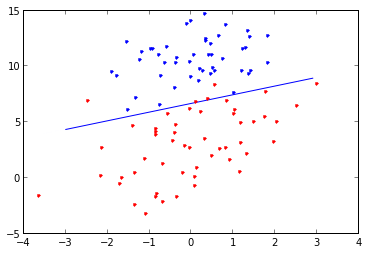
\includegraphics[width=0.7\textwidth]{logreg_files/logreg_fig_01.png}
\par
\end{center}
\end{codeoutput}
\end{codecell}
Ustteki kod bir dongu icinde belli bir $x$ noktasindan baslayarak
gradyan inisi yapti ve optimal $\theta$ degerlerini, yani regresyon
agirliklarini (weights) hesapladi. Sonra bu agirliklari bir ayrac olarak
ustte grafikledi. Ayracin oldukca iyi degerler buldugu belli oluyor.

Rasgele Gradyan Cikisi (Stochastic Gradient Ascent)

Acaba $\theta$'yi guncellerken daha az veri kullanmak mumkun mu? Yani
yon hesabi icin surekli tum veriyi kullanmasak olmaz mi?

Olabilir. Guncellemeyi sadece tek bir veri noktasi kullanarak
yapabiliriz. Yine gradyani degistirmis oluruz, sadece azar azar degisim
olur, fakat belki de bu sekilde sonuca daha cabuk ulasmak mumkun
olacaktir.

Kodlama acisindan, $\theta$ guncellemesi icin buldugumuz formulu tek
nokta bazinda da vermistik. O zaman o tek noktayi sirayla alip
guncellersek, otomatik olarak yeni bir sekilde gradyan cikisi yapmis
oluruz.

\begin{codecell}
\begin{codeinput}
\begin{lstlisting}
def stoc_grad_ascent0(data_mat, label_mat):
    m,n = data_mat.shape
    label_mat=label_mat.reshape((m,1))
    alpha = 0.01
    theta = ones((n,1))
    for i in range(m):
        h = sigmoid(sum(dot(data_mat[i],theta)))
        error = label_mat[i] - h
        theta = theta + alpha * data_mat[i].reshape((n,1)) * error
        theta = theta.reshape((n,1))
    return theta

theta = np.array(stoc_grad_ascent0(array(data),array(labels).T ))
theta.T
\end{lstlisting}
\end{codeinput}
\begin{codeoutput}
\begin{verbatim}
array([[ 1.01702007,  0.85914348, -0.36579921]])
\end{verbatim}
\end{codeoutput}
\end{codecell}
\begin{codecell}
\begin{codeinput}
\begin{lstlisting}
plot_theta(theta)

\end{lstlisting}
\end{codeinput}
\begin{codeoutput}
\begin{center}
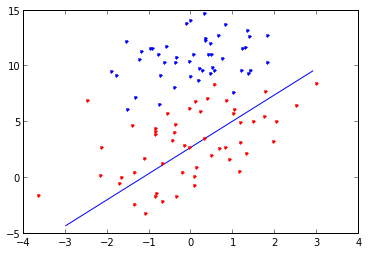
\includegraphics[width=0.7\textwidth]{logreg_files/logreg_fig_02.png}
\par
\end{center}
\end{codeoutput}
\end{codecell}
Neredeyse isimiz tamamlandi. Ustteki grafik pek iyi bir ayrac
gostermedi. Niye? Problem cok fazla salinim (oscillation) var, yani
degerler cok fazla uc noktalar arasinda gidip geliyor. Ayrica veri
noktalarini sirayla isliyoruz, veri tabii ki rasgele bir sekilde
siralanmis olabilir, ama siralanmamissa, o zaman algoritmaya raslantisal
noktalari vermek icin kod icinde zar atmamiz lazim. Metotun ismi
``rasgele (stochastic)'' gradyan cikisi, bu rasgelelik onemli. 2.
problemi duzeltmek icin yapilacak belli, 1. problem icin $\alpha$ degeri
her dongude belli oranda kucultulerek (yani $\alpha$ artik sabit degil)
sonuca yaklasirken oradan buraya savrulmasini engellemis olacagiz. Yeni
kod altta,

\begin{codecell}
\begin{codeinput}
\begin{lstlisting}
def stoc_grad_ascent1(data_mat, label_mat):
    m,n = data_mat.shape
    iter = 150
    label_mat=label_mat.reshape((m,1))
    alpha = 0.01
    theta = ones((n,1))
    for j in range(iter):
        data_index = range(m)
        for i in range(m):
            alpha = 4/(1.0+j+i)+0.0001  
            rand_index = int(random.uniform(0,len(data_index)))
	    h = sigmoid(sum(dot(data_mat[rand_index],theta)))
            error = label_mat[rand_index] - h
            theta = theta + alpha * data_mat[rand_index].reshape((n,1)) * error
            theta = theta.reshape((n,1))
    return theta

theta = np.array(stoc_grad_ascent1(array(data),array(labels).T ))
theta.T

\end{lstlisting}
\end{codeinput}
\begin{codeoutput}
\begin{verbatim}
array([[ 15.10140747,   1.16770643,  -2.06448791]])
\end{verbatim}
\end{codeoutput}
\end{codecell}
\begin{codecell}
\begin{codeinput}
\begin{lstlisting}
plot_theta(theta)

\end{lstlisting}
\end{codeinput}
\begin{codeoutput}
\begin{center}
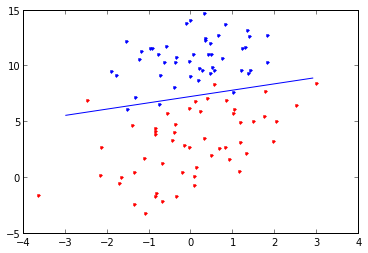
\includegraphics[width=0.7\textwidth]{logreg_files/logreg_fig_03.png}
\par
\end{center}
\end{codeoutput}
\end{codecell}
Sonuc cok iyi, ayrica daha az islemle bu noktaya eristik, yani daha az
islem ve daha hizli bir sekilde sonuca ulasmis olduk.

Tahmin (Prediction)

Elde edilen agirliklari tahmin icin nasil kullaniriz? Bu agirliklari
alip, yeni veri noktasi ile carpip sonuclari sigmoid'den gecirdigimiz
zaman bu noktanin ``1 etiketi olma olasiligini'' hesaplamis olacagiz.
Ornek (diyelim ki mevcut veri noktasi icinden bir veriyi, -mesela 15.
nokta- sanki yeniymis gibi sectik)

\begin{codecell}
\begin{codeinput}
\begin{lstlisting}
pt = df.ix[15,['intercept','x','y']]
print sigmoid(dot(array(pt), theta)), 
print "label =",labels[15]
\end{lstlisting}
\end{codeinput}
\begin{codeoutput}
\begin{verbatim}
[ 0.99999752] label = 1
\end{verbatim}
\end{codeoutput}
\end{codecell}
Oldukca yuksek bir olasilik cikti, ve hakikaten de o noktanin gercek
degeri 1 imis.

Kaynaklar

{[}1{]} http://cs229.stanford.edu/notes/cs229-notes1.pdf

{[}2{]} Harrington, P. \emph{Machine Learning in Action}

{[}3{]} Bu sekilde azar azar sonuca yaklasmaya ugrasmak tabii ki her
fonksiyon icin gecerli degildir, cunku eger fonksiyonda ``yerel
maksimumlar'' var ise, gradyan cikisi bu noktalarda takilip kalabilir (o
yerel tepelerde de birinci turev sifirlanir, gradyanin kafasi karisir).
Gradyan metotunun kullanmadan once fonksiyonumuzun tek (global) bir
maksimumu olup olmadigini dusunmemiz gerekir. Fakat sanliyiz ki olurluk
fonksiyonu tam da boyle bir fonksiyondur (sans degil tabii, bu ozelligi
sebebiyle secildi). Fonksiyon icbukeydir (concave), yani tek bir tepe
noktasi vardir. Bir soru daha: olurlugun icbukey oldugunu nasil anladik?
Fonksiyona bakarak pat diye bunu soylemek mumkun, degiskenlerde polinom
baglaminda kupsel ve daha ustu seviyesinde ustellik yok, ayrica $\log$,
$\exp$ icbukeyligi bozmuyor.

\end{document}
